%
% File w266_paper.tex
%
%% Based on the style files for ACL 2020, which were
%% Based on the style files for ACL 2018, NAACL 2018/19, which were
%% Based on the style files for ACL-2015, with some improvements
%%  taken from the NAACL-2016 style
%% Based on the style files for ACL-2014, which were, in turn,
%% based on ACL-2013, ACL-2012, ACL-2011, ACL-2010, ACL-IJCNLP-2009,
%% EACL-2009, IJCNLP-2008...
%% Based on the style files for EACL 2006 by 
%%e.agirre@ehu.es or Sergi.Balari@uab.es
%% and that of ACL 08 by Joakim Nivre and Noah Smith

\documentclass[11pt,a4paper]{article}

\usepackage[hyperref]{w266_paper}
\usepackage{times}
\usepackage{latexsym}
\usepackage{graphicx}
\renewcommand{\UrlFont}{\ttfamily\small}

% This is not strictly necessary, and may be commented out,
% but it will improve the layout of the manuscript,
% and will typically save some space.
\usepackage{microtype}

%\aclfinalcopy % Uncomment this line for the final submission
%\def\aclpaperid{***} %  Enter the acl Paper ID here

%\setlength\titlebox{5cm}
% You can expand the titlebox if you need extra space
% to show all the authors. Please do not make the titlebox
% smaller than 5cm (the original size); we will check this
% in the camera-ready version and ask you to change it back.

\newcommand\BibTeX{B\textsc{ib}\TeX}

\title{A Look at Question Answering Problem - as an Embedding based Retrieval}

\author{First Author \\
  Affiliation / Address line 1 \\
  Affiliation / Address line 2 \\
  Affiliation / Address line 3 \\
  \texttt{email@domain} \\\And
  Second Author \\
  Affiliation / Address line 1 \\
  Affiliation / Address line 2 \\
  Affiliation / Address line 3 \\
  \texttt{email@domain} \\}

\date{}

\begin{document}
\maketitle
\begin{abstract}
Here we attempt to solve a Question Answering (QA) system problem as a information retrieval problem. We derived inspiration from Overveiw QA pipeline described in Bithiah Yuan [4] thesis work. In this thesis, to select relevant answers from a larger answer set the author employs a two step process that used non-factoid answer selection using inverted index retrieval scheme to gather a set of candidates from the answer set and subsequently the author used pretrained transformers to pick most relevant answer from the candidates. Though this approach is impressive and produced some interesting results. In the above approach the non-factoid selection require some word matches for a answer to be in the potential answer list. This approach may fail to pick answers that have semantic relevance but have no words in common. In this paper we would like to employ 3 following approaches: (1) a pure informational retrieval (IR) based approach that uses TF-IDF (our baseline model) [6], (2) Yuan's Overview QA pipeline using BERT transformer [4], and (3) A Two-tower model that uses the question and answer towers. Finally we have analyzed our results with rank aware metrics[8].


\end{abstract}

\section{Introduction}

QA systems have become very prevalent in assisting customer facing or frontline workforce of large institutions to answer or advise their clients. In order to answer questions and to provide prompt andvaluable guidance and suggestions for their clienteles'  customer support personnels have a need to provide textual passages
with answers based on the knowledge base. The knowledge base could include some textual passages, letters, notes, multi-page documents, FAQs, etc. However, retrieving relevant materials from this knowledge base or information troves in a real-time or near real-time pose a serious challenge since the experience levels of the customer suppoert personnels results in inconsistent interpretations of the reports. Moreover, the large magnitude of detailed and technically written incoming reports are infeasible to read through even for the best and most experienced client facing employees. As a result, the application of QA in any domain is critical due to the highly competitive and profitable nature of the industry. Since QA research targeting a dataset or a domain that is fairly under explored can result in large profits and competitive advantages with even a slight improvements in the process. With recent advancements in NLP and Deep Learning approaches and a need for a novel QA system reinforces our motivation and has culminated in this research.

\section{Related Work}
\label{sec:length}

This research is not a first of its kind. We surveyed the literature and we found some very interesting related papers. Maia et.al [1] and Bithiah Yuan [4] used pairwise learning. While Maia et.al. did a comparative study that leveraged question context on pairwise learning, Bithiah Yuan focused on financial non-factoid answer selection and retrieved a  set of passage-level texts and selected the most relevant as the answer. Zhiyu Chen et.al. [3] performed numerical reasoning over financial data. Suman et. al. [5] provided a simplified approach and used SQuAD dataset to demonstrate their approach. Zhuang Liu et. al. [2] presented a domain specific language model pre-trained on large-scale financial corpora that enabled the capture of language knowledge and semantic information.

Our goal is to deliver a product that will help financial advisors to answer questions based on financial reports and/or disclosures. Often, there are inconsistencies and ambiguities in human interpretation. The outcome of our project will supplement FAQs automation, Chatbox, and dialog systems pertinent to the financial domain


\section{Our work}
We will try the following three approaches (1) The classical retrieval approach (our baseline) approach, (2) QA Pipeline approach [4], and (3) Two tower model approach. In the classical retrieval approach we employ the inverted index lookup like lucene to identify the relevant answer for a provided question



\subsection{Baseline approach}
\label{sect:pdf}
Our first baseline system, is an IR approach that uses a simple weighted inverted index system based on TF-IDF. TF-IDF computes the importance factor by computing the product of a term’s frequency (TF) and the inverse document frequency (IDF). Our Answer Retriever uses Anserini’s [7] a BM25 implementation to retrieve 50 candidate answers for each question. Anserini is an open-source IR toolkit built on top of Lucene (SimpleSearcher). We use the list of answers from the FiQA dataset to first build an inverted index, then we use Pyserini, a Python interface of Anserini, to generate the candidate answers.

\subsection{QA Pipeline approach}
Overview of Yuan's [4] QA pipeline. The inverted index retriever first returns the top k candidate answers. We used the pretrained BERT model with the general corpus and by fine tuning the pretrained BERT model to the target FiQA dataset. We passed the output of the BERT model to a softmax layer to assign a probability for each of the selected k answers and finally we will output the top n images within the selected k images.

\begin{figure}
  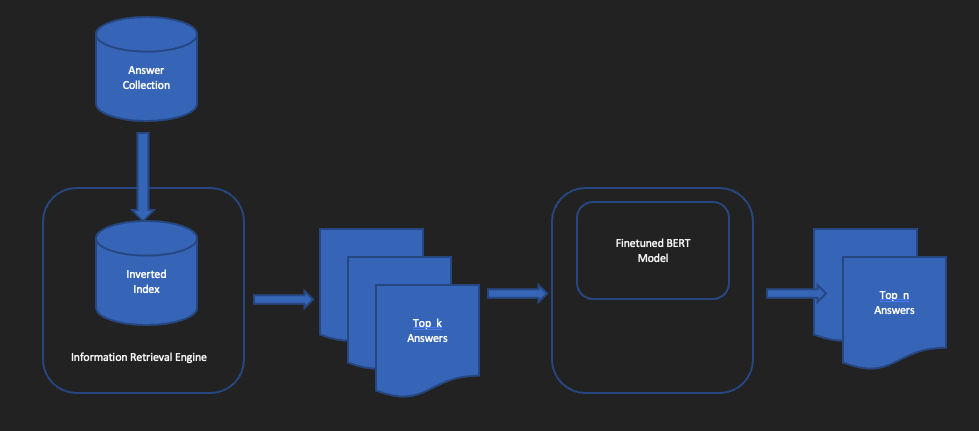
\includegraphics[width=\linewidth]{baseline.png}
  \caption{Baseline Model.}
  \label{fig:baseline model}
\end{figure}

\subsection{Two Tower Approach}
The overview of the two tower architecture is shown in Fig. 2. It has a separate question tower and an answer tower with a final dot product that computes the relavance between a given question and an answer. The answer tower takes the features from the given answer and generates an answer embedding for it. The features here are the encodings for the words found in the answer. Similarly, the question tower takes the encodings for the words in the question.  Finally, we do a simple dot product based on the two embeddings as a measure of how likely the pairs are relevant. So, basically we trained the network for each positive question and answer combination such that we maximize the dot product measure. At the end of the training we will have embeddings for each answer and question. We took the answer embeddings and load into a embedding space so that we could lookp the answer for any given question embedding. We used the ScaNN module to do the embedding similarity. The following are some important steps in this approach (check the provided notebook for details): (i) Training Step,  (ii) Model Evaluation step, (iii) Create ScaNN Index for the answer embeddings, (iv) ScaNN index lookup to obtain candidates and candidates scores for a given question. 


\begin{figure}
  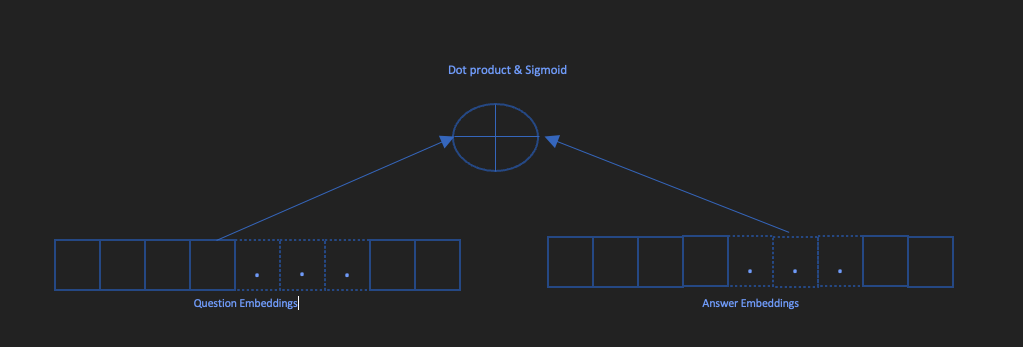
\includegraphics[width=\linewidth]{two-tower.png}
  \caption{Two Tower Model.}
  \label{fig:two-tower model}
\end{figure}


\section{Dataset}
We have used the FiQA 2018 open challenge dataset for our experiments. The FiQA 2018 open challenge collection is based on the use of unstructured text documents from different financial open data sources in English. This data comes in two flavors (a) Task 1: sentiment analysis train, and (b) Task 2: Opinion-based QA. We are interested only in the QA dataset in task 2 collection. In the dataset, for each question we have one or many relevant answers in no specific order. So, we have assumed all answers as equally relevant. For our baseline approach above, We take the list of answers from the FiQA dataset to build an inverted index. We then use the Python interface of Anserini to map 50 candidate answers for each question. Thus for each question in the dataset we have the answers as provided in the dataset and the 50 candidate answers as mapped by the Anserini. As shown below we have 6315 training questions and 333 testing questions. For each data sample we will have a question, its corresponding answers and questions' Anserini candidates.

\begin{figure}
  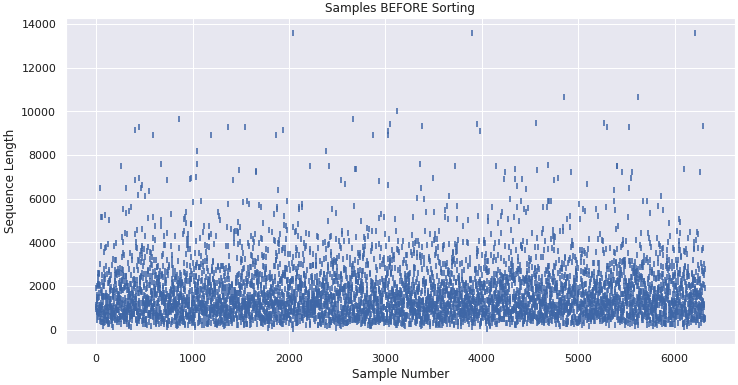
\includegraphics[width=\linewidth]{doc_size_distribution.png}
  \caption{Plot showing the # of sample (question, answer) pairs and their sequence lengths distribution.}
  \label{fig:Sequence Length Distribution}
\end{figure}

\begin{center}
\begin{tabular}{||c c ||} 
 \hline
 \textbf{} & \textbf{Questions} \\ [0.5ex] 
 \hline\hline
 \textbf{Training} & 6315 \\ 
 \hline
 \textbf{Testing} & 333 \\
 \hline

 \hline
\end{tabular}
\captionof{table}{Dataset}
\end{center}

\section{Metrics}
In order to compare and contrast our approches, we used a test set extracted from the FiQA dataset. We used the Mean Reciprocal Rank (MRR), Mean Average Precision (MAP), and Normalized Discounted Cumulative Gain (NDCG) for the top 10 answers to evaluate the systems’ performances. 


\section{Experiments}
Unlike the QA Pipeline and the Two Tower approches, the baseline approach is not a model based. The baseline approach uses a simple weighted inverted index system based on TF-IDF. So basically we could have run the metrics on both test or train data. However, for fairness we chose the test dataset to calculate the above metrics. For each data sample we will evaluate the candidates against the answers to measure the Average Precision (AP), Reverse Rank (RR) and Commulative Gain (CG).

\paragraph{}
In the case of Two Tower model as outlined above, for each data sample we looked up the candidates and candidate scores from the ScaNN index. Similarly, as in the case of baseline approach, We will evaluate the candidates against the answer to generate AP, RR and CG scores for each data sample.

\paragraph{}
We had run our experiments with different sequence lengths for the overview pipeline and two tower approaches respectively. We have plotted the metrics in figures 3 and 4.

\section{Results}
As shown in table 2, MRR and MAP scores have shown considerably improved with the two tower model as opposed to the baseline and NDCG scores showed a 5 percentage point improvement at embedding size 128. From the two tower approach plot shown in figure 4 we see a linear fall off in the MRR score with the increase in embedding size where as the NDCG score show a slight fall with the embedding size between 50 and 275 and show a considerable improvement there after. 


\begin{center}
\begin{tabular}{||c c c c||} 
 \hline
 \textbf{Approach} & \textbf{MRR} & \textbf{MAP} & \textbf{NDCG} \\ [0.5ex] 
 \hline\hline
 \textbf{Baseline} & 0.2943 & 0.2810 & 0.7067 \\ 
 \hline
 \textbf{QA Pipeline} & - & - & - \\
 \hline
 \textbf{Two Tower} & 0.57357 & 0.57357 & 0.76978 \\
 \hline

 \hline
\end{tabular}
\captionof{table}{Approaches and scores (Two Tower with 128 Embedding Sz.)}
\end{center}

\begin{figure}
  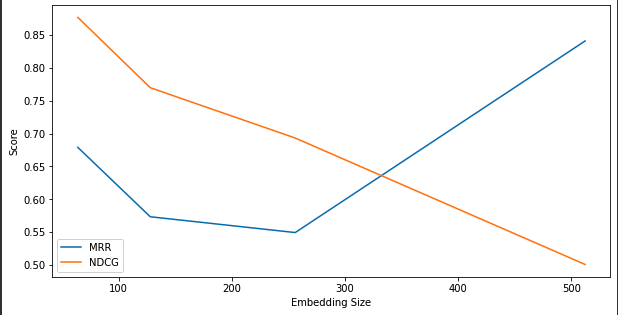
\includegraphics[width=\linewidth]{metric_plot.png}
  \caption{Score vs. Embedding Sz. plot for two-tower}
  \label{fig:two-tower model}
\end{figure}


\section{Limitations}
The two tower and overview pipeline approaches not only lend naturally match answers with semantic relevance even when there is very little word overlap between answers and questions it also perform overall in accuracy performance. However, these methods grow prohibitively in time complexity with the increase in embedding size. So matching relevant documents becomes a challenge with the increase in document size. For our experimental dataset sequence length of 512 reasonably covers the text however the data with moderate or large sized documents this method could slow down drastically. 

\section{Future work}
We have measured mean average precision (MAP), normalized discounted cummulative gain (NCDG) score


\section{conclusion}
Papers that have been or will be submitted to other meetings or publications must indicate this at submission time in the START submission form, and must be withdrawn from the other venues if accepted by ACL 2020. Authors of papers accepted for presentation at ACL 2020 must notify the program chairs by the camera-ready deadline as to whether the paper will be presented. We will not accept for publication or presentation the papers that overlap significantly in content or results with papers that will be (or have been) published elsewhere.



\section*{Acknowledgments}

First and foremost, we would like to thank our instructors Prof. Mark Butler, and Prof. Natalie for their valuable time and feedback. We are very grateful for their encouragement through out this course.

%\bibliographystyle{acl_natbib}
%\bibliography{antholog, w266_paper}

\begin{thebibliography}{}

\bibitem{Maia21} Macedo Maia, and Markus Endres \emph{A comparative study using different question context information on pairwise learning-to-rank CQA transformer models in the home improvement domain}, Journal of Data Intelligence, Vol. 3, No. 1 (2021) 131–148

\bibitem{Liu20} Zhuang Liu , Degen Huang, Kaiyu Huang, Zhuang Li and Jun Zhao \emph{FinBERT: A Pre-trained Financial Language Representation Model for Financial Text Mining}, Proceedings of the Twenty-Ninth International Joint Conference on Artificial Intelligence (IJCAI-20) Special Track on AI in FinTech

\bibitem{Chen21} Zhiyu Chen, Wenhu Chen, Charese Smiley, Sameena Shah, Iana Borova, Dylan Langdon, Reema Moussa, Matt Beane, Ting-Hao Huang, Bryan Routledge and William Yang Wang, \emph{FINQA: A Dataset of Numerical Reasoning over Financial Data}, 2021.

\bibitem{Yuan20} Bithiah Yuan, \emph{FinBERT-QA: Financial Question Answering with pre-trained BERT Language Models}, Master’s Thesis, Albert-Ludwigs-University Freiburg, Faculty of Engineering, Department of Computer Science, 2020.

\bibitem{Karanjit21} Suman Karanjit, \emph{Question and Answering Using BERT}, Computer Science Major Minnesota State University Moorhead, 2021.

\bibitem{Manning19} Christopher Manning and Pandu Nayak. Information Retrieval and Web Search. 2019. url: https://web.stanford.edu/class/cs276/.

\bibitem{Yang17} Peilin Yang, Hui Fang, and Jimmy Lin. \emph{Anserini: Enabling the Use of Lucene for Information Retrieval Research}. In: Proceedings of the 40th International ACM SIGIR Conference on Research and Development in Information Retrieval, Shinjuku, Tokyo, Japan, August 7-11, 2017. Ed. by Noriko Kando et al. ACM, 2017, pp. 1253–1256. doi: 10.1145/3077136.3080721. url: https://doi.org/ 10.1145/3077136.3080721.

\bibitem{Taifi19} Moussa Taifi, \emph{MRR vs MAP vs NDCG: Rank-Aware Evaluation Metrics And When To Use Them}, https://medium.com/swlh/rank-aware-recsys-evaluation-metrics-5191bba16832

\end{thebibliography}



\appendix

\section{Appendices}
\label{sec:appendix}
Appendices are material that can be read, and include lemmas, formulas, proofs, and tables that are not critical to the reading and understanding of the paper. 
Appendices should be \textbf{uploaded as supplementary material} when submitting the paper for review.
Upon acceptance, the appendices come after the references, as shown here.


\end{document}
